\documentclass[10pt,firamath,cours]{nsi}



\begin{document}
\chapter{BDD partie 4}
\section{Requêtes SQL}
\subsection{Requête et résultat}
Une requête est une commande SQL et renvoie une table.\\
On se replace dans le contexte du chapitre précédent.

\subsection{Sélection d'attributs}
\begin{minted}{sql}
SELECT nom, prenom
FROM Auteur;
    \end{minted}

\begin{center}
    \tabstyle[UGLiOrange]
    \begin{tabular}{c|c}
        \ccell nom  & \ccell prenom \\
        Ammaniti    & Niccolo       \\
        Avallone    & Silvia        \\
        Camus       & Albert        \\
        Hamilton    & Peter         \\
        Hugo        & Victor        \\
        Murgia      & Michela       \\
        Rhode james & Montague      \\
        Tolkien     & John
    \end{tabular}
\end{center}


\subsection{Sélection de tous les attributs}
\begin{minted}{sql}
SELECT *
FROM Auteur;
    \end{minted}

\begin{center}
    \tabstyle[UGLiOrange]
    \begin{tabular}{c|c|c|c|c}
        \ccell id\_auteur & \ccell nom\_pays & \ccell nom  & \ccell prenom & \ccell date\ naissance \\
        1                 & France           & Hugo        & Victor        & 1802-02-26             \\
        2                 & France           & Camus       & Albert        & 1913-11-07             \\
        4                 & Italie           & Avallone    & Silvia        & 1948-04-13             \\
        5                 & Italie           & Ammaniti    & Niccolo       & 1966-09-25             \\
        6                 & Italie           & Murgia      & Michela       & 1972-06-03             \\
        7                 & Royaume-Uni      & Hamilton    & Peter         & 1960-03-02             \\
        8                 & Royaume-Uni      & Tolkien     & John          & 1892-01-03             \\
        9                 & Royaume-Uni      & Rhode James & Montague      & 1862-08-01
    \end{tabular}
\end{center}


\subsection{Sélection avec condition}
\begin{minted}{sql}
SELECT nom, date_naissance
FROM Auteur
WHERE date(date_naissance) < '1900';
    \end{minted}

\begin{center}
    \tabstyle[UGLiOrange]
    \begin{tabular}{c|c}
        \ccell nom  & \ccell date\_naissance \\
        Hugo        & 1802-02-16             \\
        Tolkien     & 1892-01-03             \\
        Rhode James & 1862-08-01             \\
    \end{tabular}
\end{center}


\subsection{Sélection avec conditions multiples}
\begin{minted}{sql}
SELECT nom, date_naissance
FROM Auteur
WHERE date(date_naissance) < '1900'
  AND nom_pays = 'France';
    \end{minted}

\begin{center}
    \tabstyle[UGLiOrange]
    \begin{tabular}{c|c}
        \ccell nom & \ccell date\_naissance \\
        Hugo       & 1802-02-16             \\
    \end{tabular}
\end{center}


\subsection{Renommer les colonnes}
\begin{minted}{sql}
SELECT titre AS Titre_ouvrage, num_isbn AS Reference_ISBN
FROM Livre
WHERE date(annee) > '2015';
\end{minted}

\begin{center}
    \tabstyle[UGLiOrange]
    \begin{tabular}{c|c}
        \ccell Titre\_ouvrage & \ccell Reference\_ISBN \\
        les misérables        & 9782072730672          \\
        et je t'emmène        & 9782221133651          \\
        d'acier               & 9782867465987          \\
        salvation             & 9791093835334          \\
    \end{tabular}
\end{center}

\subsection{Fonction COUNT}
\begin{minted}{sql}
SELECT COUNT(titre) AS Nb_Livres_avant_2015
FROM Livre
WHERE annee < 2015;    
\end{minted}

\begin{center}
    \tabstyle[UGLiOrange]
    \begin{tabular}{c}
        \ccell Nb\_Livres\_avant\_2015 \\
        4
    \end{tabular}
\end{center}

\subsection{Autres fonctions similaires}
Fonctions MIN, MAX, SUM et AVG (moyenne).

\subsection{\'Eliminer les doublons}
Sans élimination :
\begin{minted}{sql}
SELECT id_auteur
FROM Ecrire;
    \end{minted}

\begin{center}
    \tabstyle[UGLiOrange]
    \begin{tabular}{c}
        \ccell id\_auteur \\
        1                 \\
        1                 \\
        2                 \\
        4                 \\
        5                 \\
        6                 \\
        7                 \\
        8                 \\
        9
    \end{tabular}
\end{center}

Avec élimination :
\begin{minted}{sql}
SELECT DISTINCT id_auteur
FROM Ecrire;
    \end{minted}

\begin{center}
    \tabstyle[UGLiOrange]
    \begin{tabular}{c}
        \ccell id\_auteur \\
        1                 \\
        2                 \\
        4                 \\
        5                 \\
        6                 \\
        7                 \\
        8                 \\
        9
    \end{tabular}
\end{center}
\subsection{Ordonner les tuples}
Ordonner les noms dans l'ordre croissant :
\begin{minted}{sql}
SELECT nom,prenom FROM Auteur
ORDER BY nom ASC;
    \end{minted}

\begin{center}
    \tabstyle[UGLiOrange]
    \begin{tabular}{c|c}
        \ccell nom  & \ccell prenom \\
        Ammaniti    & Niccolo       \\
        Avallone    & Silvia        \\
        Camus       & Albert        \\
        Hamilton    & Peter         \\
        Hugo        & Victor        \\
        Murgia      & Michela       \\
        Rhode james & Montague      \\
        Tolkien     & John
    \end{tabular}
\end{center}
Pour l'ordre décroissant on utilise \mintinline{sql}{DESC}.


\section{Jointures}
\subsection{Principe}
Considérons 2 tables T1 et T2 et supposons que c est une clé étrangère qui fait référence à b.

\begin{center}
    \tabstyle[UGLiOrange]
    \begin{tabular}{c|c}
        \ccell a & \ccell b \\
        0        & 0        \\
        0        & 1        \\
        1        & 1        \\
        2        & 1        \\
        3        & 2        \\
        4        & 5 
    \end{tabular}\hspace{3em}
    \begin{tabular}{c|c}
        \ccell c & \ccell d \\
        0        & 10       \\
        0        & 30       \\
        1        & 12       \\
        2        & 100      \\
        2        & 200 
    \end{tabular}
\end{center}

Voici table qui est la \textit{jointure} T1 et T2 selon la condition b=c :


\begin{center}
    \tabstyle[UGLiOrange]
\begin{tabular}{c|c|c|c}
    \ccell a & \ccell b & \ccell c & \ccell d \\
    0        & 0        & 0        & 10       \\
    0        & 0        & 0        & 30       \\
    0        & 1        & 1        & 12       \\
    1        & 1        & 1        & 12       \\
    2        & 1        & 1        & 12       \\
    3        & 2        & 2        & 100      \\
    3        & 2        & 2        & 200      \\
\end{tabular}
\end{center}
C'est la table obtenue en faisant correspondre chaque tuple de T1 avec chaque autre tuple de T2 tel que b et c soient égaux.

\subsection{Applications}
Produire la table des noms des auteurs venant de pays de plus de 61 millions d'habitants :
\begin{minted}{sql}
SELECT nom
from Auteur
         JOIN Pays ON Auteur.nom_pays = Pays.nom_pays
WHERE population > 62000000;
    \end{minted}

    \begin{center}
        \tabstyle[UGLiOrange]
    \begin{tabular}{c}
        \ccell nom \\
        Hugo\\
        Camus\\
        Avallone\\
        Ammaniti\\
        Murgia
    \end{tabular}
    \end{center}



Produire la table des noms et prénoms des auteurs ayant écrit un livre dont le titre comporte « la»  :
\begin{minted}{sql}
SELECT DISTINCT nom, prenom
FROM Auteur
         JOIN Ecrire ON Ecrire.id_auteur = Auteur.id_auteur
         JOIN Livre ON Livre.num_isbn = Ecrire.num_isbn
WHERE Livre.titre LIKE '%la%';
\end{minted}

\begin{center}
    \tabstyle[UGLiOrange]
\begin{tabular}{c|c}
    \ccell nom & \ccell prenom\\
    Camus & Albert \\
    Rodhe James & Montague
\end{tabular}
\end{center}

\section{Mises à jour}


\subsection{INSERT INTO}
Insérer un nouveau tuple dans la table \textbf{Auteur} :
\begin{minted}{sql}
INSERT INTO Auteur VALUES
    (128,'France','Leleu','Frédéric','1974-05-16');
\end{minted}

Les colonnes doivent être dans le même ordre qu'à la création, sinon utiliser
\begin{minted}{sql}
INSERT INTO Auteur VALUES (nom,id_auteur)
    ('Leleu',128);
\end{minted}

Les colonnes non renseignées prendront par défaut la valeur \mintinline{sql}{NULL} ce qui peut poser problème.


\subsection{DELETE}

Supprimer les tuples de \textbf{Ecrire} dont l'auteur a l'id\_auteur 1:
\begin{minted}{sql}
DELETE FROM Ecrire WHERE id_auteur = 1;
\end{minted}

Penser aux contraintes de références (clé étrangères) : si on supprime un tuple et qu'un tuple d'une autre table fait référence à celui qu'on supprime, cela provoquera une erreur.


\subsection{UPDATE}

Mettre à jour l'id du tuple de \textbf{Auteur} dont le nom est Hugo
\begin{minted}{sql}
UPDATE Auteur
SET id_auteur = 1024
WHERE nom = 'Hugo';
	\end{minted}

Penser aux contraintes de références (clé étrangères) lors de la mise à jour.
\section{Exercices}

\begin{exercice}[ : Prix Nobel]
    \begin{center}
        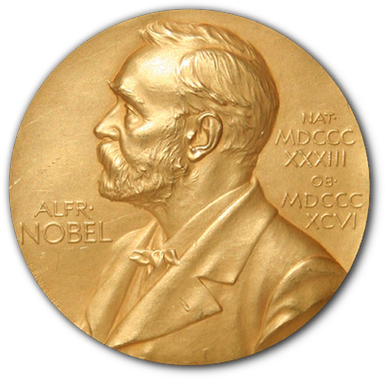
\includegraphics[width=5cm]{img/nobel}
    \end{center}
    \textbf{Premier contact}\\
    
    Avec un éditeur de texte ouvir le fichier \texttt{create\_nobel.sql}.\\
    En explorant la structure de la base de données, répondez aux questions suivantes :	\\
    \begin{enumerate}
        \item 	Combien de tables possède la base de données ?
        \item 	Combien d'attributs possède la table Nobel ?
        \item 	Quel est le type de l'attribut annee ?\\
    \end{enumerate}
    \textbf{La table Nobel}\\
    
    Importer ce fichier dans DB Browser pour créer la BDD \texttt{nobel.db}.\\
    En explorant les données de la table Nobel, répondez aux questions suivantes :\\
    
    \begin{enumerate}
        \setcounter{enumi}{3}
        \item 	Combien d'enregistrements possède la table Nobel ?
        \item 	Dans quelle discipline Paul Krugman est-il devenu Prix Nobel ?
        \item 	En quelle année Albert Fert a-t-il eu le prix Nobel ?	\\
    \end{enumerate}

    \textbf{Requêtes d'interrogation}\\
    
    En utilisant l'onglet : « Exécuter le SQL », indiquez le code SQL permettant de répondre aux questions suivantes :\\
    
    \begin{enumerate}
            \setcounter{enumi}{6}
    \item  Comment afficher le nom de tous les lauréats en évitant les doublons ? (809 enregistrements)
    \item Comment afficher le nom de toutes les disciplines en évitant les doublons ? (6 enregistrements)
    \item  Quelle est la discipline de Wilhelm Conrad Röntgen ? (1 enregistrement)
    \item  Dans quelle discipline Paul Krugman est-il devenu Prix Nobel ? (1 enregistrement)
    \item  En quelle année Albert Fert a-t-il eu le prix Nobel ? (1 enregistrement)
    \item  Quelle est l'année de distinction de Pierre Curie ? (1 enregistrement)
    \item  Quelle est l'année de distinction et la matière de Bertha von Suttner ? (1 enregistrement)
    \item  Quels sont les lauréats distingués au XXI e siècle ? (97 enregistrements)
    \item  Quels sont les lauréats du prix Nobel de la Paix durant la deuxième guerre mondiale ? (2 enregistrements)
    \item  Quels sont les lauréats distingués en Médecine en 1901 et en 2001 ? (4 enregistrements)
    \item  Quels sont les lauréats des prix nobel de Physique et de Médecine en 2008 ? (3 enregistrements)	\\
    \end{enumerate}
    
    \textbf{Requêtes d'agrégation}\\
    
    \begin{enumerate}
    \setcounter{enumi}{17}
    \item  Combien d'enregistrements au total comporte la table ? (816 enregistrements)
    \item  Combien de personnes ont reçu le prix Nobel de la paix ? (119 enregistrements)
    \item  Combien de personnes ont reçu le prix Nobel de littérature ? (105 enregistrements)
    \item  Combien de personnes ont reçu le prix Nobel de mathématiques ? (0 enregistrements)
    \item  Combien de personnes ont reçu un prix Nobel en 1901 ? (6 enregistrements)
    \item  Combien de personnes ont reçu un prix Nobel de chimie en 1939 ? (2 enregistrements)
    \item  En quelle année a été décerné le premier prix Nobel d'économie ? (Réponse : 1969)
    \item  Combien de prix Nobel a reçu Marie Curie ? (Réponse : 2)
    \item  Quels sont les prix lauréats, leur discipline et l'année de distinction de tous les prix Nobel contenant cohen dans leur nom (on ne fera pas de distinction de casse) ? (2 enregistrements)
    \item  Combien y a-t-il eu de lauréats en Physique et en Chimie ? (335 enregistrements)
    \item  Combien y a-t-il eu de lauréats de Médecine et de littérature en 2000 ? (4 enregistrements)
    \item  Nombre de lauréats différents parmi les prix Nobel de la paix ? (116 enregistrements)\\
    \end{enumerate}
    
    \textbf{Requêtes de mise à jour}\\
    \setcounter{enumi}{29}
    En utilisant l'onglet Exécuter le SQL, indiquez le code SQL permettant de répondre aux questions suivantes :\\
    
    \begin{enumerate}
    \item En 2019, Esther Duflo a reçu le prix Nobel d'économie. Écrivez la requête permettant d'insérer cet enregistrement.
    \item  Quelle requête permet de modifier l'enregistrement précédent pour accoler le nom d'époux (Banerjee) après celui de Duflo ?
    \item   De nombreuses pétitions circulent pour retirer le prix Nobel à Aung San Suu Kyi. Quelle requête permettrait cela ?
    \end{enumerate}
    \end{exercice}
    
    
    
  
    
    
    \begin{exercice}[ : JO]
    Nous allons travailler sur une base de données liée aux Jeux Olympiques de Londres qui ont eu lieu en 2012.\\
    \begin{center}
        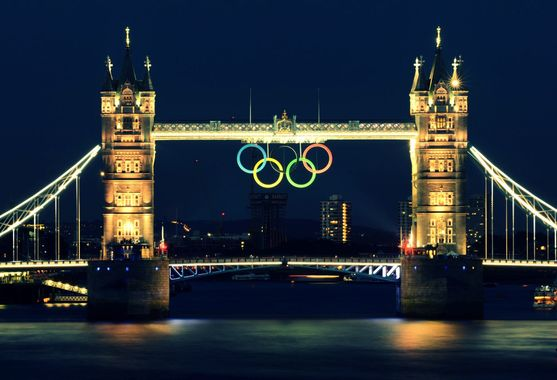
\includegraphics[width=8cm]{img/jo_london}
    \end{center}
    
    \textbf{\large Partie 1 : \'Etude du schéma relationnel}\\
    
    Avec un éditeur de texte tout simple, ouvrir le fichier \texttt{create\_JO.sql}, regarder les lignes qui définissent les différentes tables de la BDD et donner sous forme écrite son schéma relationnel en soulignant clés primaires (en trait plein) et clés étrangère (en pointillés).\\
    
    \textbf{\large Partie 2 : Requêtes SQL}\\
    
    Avant toute chose, ouvrir DB Browser, importer le fichier \texttt{create\_JO.sql} pour créer la BDD \texttt{JO.db}.\\
    Ensuite exécuter les bonnes requêtes SQL pour obtenir les données suivantes.\\
    
    \textbf{Requêtes sans jointures}
    \begin{enumerate}
        \item 	Afficher le nom et prénom des sportifs. Combien y en a-t-il ?
        \item 	Afficher les codes des pays dont viennent les sportifs par ordre alphabétique en éliminant les doublons.
        \item 	Afficher la liste des sportifs français (utiliser cio = 'France').
        \item 	Afficher la liste des 301 disciplines triées par l'identifiant du sport auxquelles elles se rapportent.
        \item 	Afficher les noms des 86 pays situés après la France et avant la Russie (Russia) par ordre alphabétique.\\
                Utiliser les opérateurs inférieur et supérieur. Remarquer que l'opérateur \mintinline{SQL}{BETWEEN} ne produit pas le résultat attendu (88 pays).
        \item 	Afficher les 98 identifiants de discipline dont au moins une épreuve a eu lieu entre le 27 et le 31 juillet 2012 inclus.
        \item 	Afficher les noms des 61 sportifs qui sont soit français (FRA) soit britanniques (GBR).
        \item 	Afficher les intitulés des 131 disciplines contenant la chaîne de caractères «WOMEN».
    
        \item  Donner les 3 pays (CIO, nom) dont on ne connaît pas le code ISO2 ou ISO3 (utiliser le critère \mintinline{sql}{IS NULL}).
        \item 	Donner les noms et prénoms des 2 sportifs dont le sexe est mentionné dans la BDD.
        \item  	À l'aide de la fonction \mintinline{sql}{COUNT}, donner le nombre de sports (pas la liste).
        \item  Donner le nombre de discipline(s) du sport d'identifiant 1 (pas la liste).
    
    
        \item Combien de noms de familles différents sont portés par les sportifs ?
        \item Donner le nombre de pays n'ont pas d'ISO2.
        \item Donner le nombre de médailles d'or attribués lors de ces JO.
        \item Afficher en une table le premier et le dernier évènement sportif	de ces JO.\\
    \end{enumerate}
    \textbf{Requêtes avec jointures}
    \begin{enumerate}
        \setcounter{enumi}{16}
        \item Afficher la listes des noms et prénoms des sportifs européens.
    \item Afficher la liste des disciplines dépendant de l'athlétisme.
    \item Afficher toutes jours pendant lesquels un évènement lié à l'athlétisme eu lieu.
    \item Afficher les noms, prénoms et médailles gagnées par des sportifs dont le sexe figure dans la BDD.
    \item Afficher la liste des Français médaillés d'or.
    \item Afficher les noms, prénoms, sports et disciplines des sportifs ayant obtenu une médaille d'or.
    \end{enumerate}
    
    \end{exercice}
\end{document}